\hypertarget{group__texteditors}{
\section{Text Editor Windows}
\label{group__texteditors}\index{Text Editor Windows@{Text Editor Windows}}
}


Max has a simple built-\/in text editor object that can display and edit text in conjunction with your object.  


Collaboration diagram for Text Editor Windows:\nopagebreak
\begin{figure}[H]
\begin{center}
\leavevmode
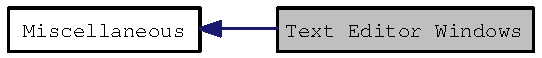
\includegraphics[width=148pt]{group__texteditors}
\end{center}
\end{figure}
Max has a simple built-\/in text editor object that can display and edit text in conjunction with your object. The routines described here let you create a text editor.

When the editor window is about to be closed, your object could receive as many as three messages. The first one, okclose, will be sent if the user has changed the text in the window. This is the standard okclose message that is sent to all \char`\"{}dirty\char`\"{} windows when they are about to be closed, but the text editor window object passes it on to you instead of doing anything itself. Refer to the section on Window Messages for a description of how to write a method for the okclose message. It’s not required that you write one—if you don’t, the behavior of the window will be determined by the setting of the window’s w\_\-scratch bit. If it’s set, no confirmation will be asked when a dirty window is closed (and no okclose message will be sent to the text editor either). The second message, edclose, requires a method that should be added to your object at initialization time. The third message, edSave, allows you to gain access to the text before it is saved, or save it yourself.

\begin{DoxySeeAlso}{See also}
\hyperlink{chapter_enhancements_chapter_enhancements_ed}{Showing a Text Editor} 
\end{DoxySeeAlso}
